
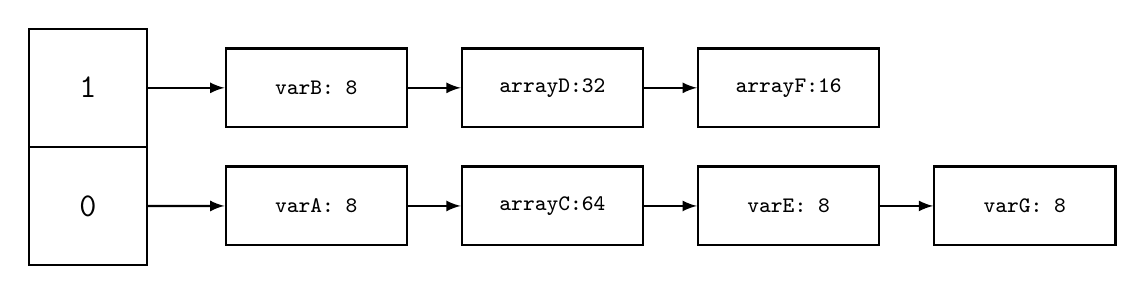
\begin{tikzpicture}[font={\fontsize{12pt}{12}\selectfont}]

    \node[rectangle, draw, color=black, thick, anchor=south west, minimum width=1.5cm, minimum height=1.5cm, inner sep=0pt] (c1) at (0, 1.5)    {\ttfamily 1};
    \node[rectangle, draw, color=black, thick, anchor=south west, minimum width=1.5cm, minimum height=1.5cm, inner sep=0pt] (c0) at (0, 0)      {\ttfamily 0};
   
    % C0 
    \node[rectangle, draw, color=black, thick, anchor=south west, minimum width=2.3cm, minimum height=1cm, inner sep=0pt] (b01) at (2.5, 0.25) {\footnotesize \verb+varA: 8+};
    \node[rectangle, draw, color=black, thick, anchor=south west, minimum width=2.3cm, minimum height=1cm, inner sep=0pt] (b02) at (5.5, 0.25) {\footnotesize \verb+arrayC:64+};
    \node[rectangle, draw, color=black, thick, anchor=south west, minimum width=2.3cm, minimum height=1cm, inner sep=0pt] (b03) at (8.5, 0.25) {\footnotesize \verb+varE: 8+};
    \node[rectangle, draw, color=black, thick, anchor=south west, minimum width=2.3cm, minimum height=1cm, inner sep=0pt] (b04) at (11.5, 0.25) {\footnotesize \verb+varG: 8+};
    \draw[-latex, thick] (c0) -- (b01);
    \draw[-latex, thick] (b01) -- (b02);
    \draw[-latex, thick] (b02) -- (b03);
    \draw[-latex, thick] (b03) -- (b04);

    % C1 
    \node[rectangle, draw, color=black, thick, anchor=south west, minimum width=2.3cm, minimum height=1cm, inner sep=0pt] (b11) at (2.5, 1.75) {\footnotesize \verb+varB: 8+};
    \node[rectangle, draw, color=black, thick, anchor=south west, minimum width=2.3cm, minimum height=1cm, inner sep=0pt] (b12) at (5.5, 1.75) {\footnotesize \verb+arrayD:32+};
    \node[rectangle, draw, color=black, thick, anchor=south west, minimum width=2.3cm, minimum height=1cm, inner sep=0pt] (b13) at (8.5, 1.75) {\footnotesize \verb+arrayF:16+};
    \draw[-latex, thick] (c1) -- (b11);
    \draw[-latex, thick] (b11) -- (b12);
    \draw[-latex, thick] (b12) -- (b13);

\end{tikzpicture}
